\documentclass[a4paper,9pt]{beamer}\usepackage[]{graphicx}\usepackage[]{color}
%% maxwidth is the original width if it is less than linewidth
%% otherwise use linewidth (to make sure the graphics do not exceed the margin)
\makeatletter
\def\maxwidth{ %
  \ifdim\Gin@nat@width>\linewidth
    \linewidth
  \else
    \Gin@nat@width
  \fi
}
\makeatother

\definecolor{fgcolor}{rgb}{0.345, 0.345, 0.345}
\newcommand{\hlnum}[1]{\textcolor[rgb]{0.686,0.059,0.569}{#1}}%
\newcommand{\hlstr}[1]{\textcolor[rgb]{0.192,0.494,0.8}{#1}}%
\newcommand{\hlcom}[1]{\textcolor[rgb]{0.678,0.584,0.686}{\textit{#1}}}%
\newcommand{\hlopt}[1]{\textcolor[rgb]{0,0,0}{#1}}%
\newcommand{\hlstd}[1]{\textcolor[rgb]{0.345,0.345,0.345}{#1}}%
\newcommand{\hlkwa}[1]{\textcolor[rgb]{0.161,0.373,0.58}{\textbf{#1}}}%
\newcommand{\hlkwb}[1]{\textcolor[rgb]{0.69,0.353,0.396}{#1}}%
\newcommand{\hlkwc}[1]{\textcolor[rgb]{0.333,0.667,0.333}{#1}}%
\newcommand{\hlkwd}[1]{\textcolor[rgb]{0.737,0.353,0.396}{\textbf{#1}}}%
\let\hlipl\hlkwb

\usepackage{framed}
\makeatletter
\newenvironment{kframe}{%
 \def\at@end@of@kframe{}%
 \ifinner\ifhmode%
  \def\at@end@of@kframe{\end{minipage}}%
  \begin{minipage}{\columnwidth}%
 \fi\fi%
 \def\FrameCommand##1{\hskip\@totalleftmargin \hskip-\fboxsep
 \colorbox{shadecolor}{##1}\hskip-\fboxsep
     % There is no \\@totalrightmargin, so:
     \hskip-\linewidth \hskip-\@totalleftmargin \hskip\columnwidth}%
 \MakeFramed {\advance\hsize-\width
   \@totalleftmargin\z@ \linewidth\hsize
   \@setminipage}}%
 {\par\unskip\endMakeFramed%
 \at@end@of@kframe}
\makeatother

\definecolor{shadecolor}{rgb}{.97, .97, .97}
\definecolor{messagecolor}{rgb}{0, 0, 0}
\definecolor{warningcolor}{rgb}{1, 0, 1}
\definecolor{errorcolor}{rgb}{1, 0, 0}
\newenvironment{knitrout}{}{} % an empty environment to be redefined in TeX

\usepackage{alltt}
%
% Choose how your presentation looks.
%
% For more themes, color themes and font themes, see:
% http://deic.uab.es/~iblanes/beamer_gallery/index_by_theme.html
%
 \mode<presentation>
{
  \usetheme{Singapore}      % or try Darmstadt, Madrid, Warsaw, ...
  \usecolortheme{} % or try albatross, beaver, crane, ...
  \usefonttheme{serif}  % or try serif, structurebold, ...
  \mode<presentation>{\useinnertheme{rounded}}
  \setbeamertemplate{navigation symbols}{}
  \setbeamertemplate{caption}[numbered]
  \addtobeamertemplate{navigation symbols}{}{%
    \usebeamerfont{footline}%
    \usebeamercolor[fg]{footline}%
    \hspace{1em}%
    %\insertfrawas done by one doctor menumber/\inserttotalframenumber
}
} 
\usepackage{float}
\usepackage{graphicx}
\usepackage{mathtools}
\usepackage{amsmath}
\usepackage[english]{babel}
\usepackage[utf8x]{inputenc}
\usepackage{color, colortbl}
\usepackage{subfig}
\usepackage{listings}
\title{Multiple Surrogates Validation}

\author{Olusoji Oluwafemi Daniel (1541893)}
\institute{Hasselt University, Belgium}
%\date{April 3, 2017}
\IfFileExists{upquote.sty}{\usepackage{upquote}}{}
\begin{document}

\frame{\maketitle}

\section{Previous Results}

\begin{frame}{Joint Modelling Results}
% latex table generated in R 3.4.0 by xtable 1.8-2 package
% Tue Jun 13 14:53:27 2017
\tiny
\begin{table}[H]
\centering
\begin{tabular}{rrrrrrrr}
  \hline
S & UN\_Assoc & ADJ\_ASSOC & Lower\_CI & Upper\_CI & S\_Trt & pval & pvaladj \\ 
  \hline
 \alert{18} & 0.90 & 0.83 & 0.56 & 0.94 & 0.52 & 0.00 & 0.04 \\ 
  \alert{29} & 0.82 & 0.57 & 0.11 & 0.83 & 0.40 & 0.00 & 0.01 \\ 
    \alert{6} & 0.29 & 0.56 & 0.10 & 0.83 & -0.11 & 0.77 & 0.92 \\ 
   \alert{15} & 0.12 & 0.46 & -0.05 & 0.78 & -0.35 & 0.44 & 0.80 \\ 
    \alert{5} & 0.14 & 0.41 & -0.11 & 0.75 & -0.45 & 0.60 & 0.88 \\ 
   \alert{14} & 0.29 & 0.32 & -0.21 & 0.70 & 0.19 & 0.65 & 0.88 \\ 
   \alert{24} & -0.18 & 0.25 & -0.28 & 0.67 & -0.36 & 0.10 & 0.52 \\ 
   \alert{22} & 0.29 & 0.23 & -0.30 & 0.65 & 0.24 & 0.48 & 0.80 \\ 
   \alert{17} & 0.27 & 0.19 & -0.34 & 0.63 & 0.56 & 0.45 & 0.80 \\ 
   \alert{26} & 0.31 & 0.19 & -0.34 & 0.62 & 0.35 & 0.34 & 0.78 \\ 
    9 & 0.33 & 0.15 & -0.37 & 0.60 & 0.67 & 0.24 & 0.65 \\ 
   23 & 0.17 & 0.12 & -0.40 & 0.58 & 0.23 & 0.66 & 0.88 \\ 
    2 & -0.34 & 0.10 & -0.42 & 0.57 & -0.86 & 0.03 & 0.26 \\ 
   19 & -0.22 & 0.10 & -0.42 & 0.56 & -0.93 & 0.17 & 0.58 \\ 
   13 & 0.44 & -0.04 & -0.52 & 0.47 & 0.61 & 0.01 & 0.11 \\ 
   28 & 0.31 & -0.05 & -0.53 & 0.46 & 0.66 & 0.08 & 0.51 \\ 
   30 & -0.18 & -0.06 & -0.54 & 0.45 & -0.52 & 0.51 & 0.80 \\ 
   25 & -0.01 & -0.08 & -0.55 & 0.43 & 0.09 & 0.85 & 0.92 \\ 
    1 & -0.23 & -0.09 & -0.56 & 0.42 & -0.37 & 0.40 & 0.80 \\ 
    8 & 0.22 & -0.10 & -0.56 & 0.42 & 0.60 & 0.16 & 0.58 \\ 
   21 & -0.03 & -0.11 & -0.58 & 0.41 & 0.10 & 0.86 & 0.92 \\ 
   16 & -0.13 & -0.12 & -0.58 & 0.40 & -0.08 & 0.77 & 0.92 \\ 
    3 & -0.23 & -0.12 & -0.58 & 0.40 & -0.35 & 0.43 & 0.80 \\ 
    7 & -0.29 & -0.13 & -0.59 & 0.39 & -0.34 & 0.31 & 0.77 \\ 
   12 & -0.10 & -0.14 & -0.59 & 0.38 & -0.01 & 0.96 & 0.96 \\ 
   20 & -0.14 & -0.19 & -0.63 & 0.34 & -0.06 & 0.93 & 0.96 \\ 
   11 & -0.05 & -0.22 & -0.64 & 0.31 & 0.10 & 0.67 & 0.88 \\ 
   10 & -0.20 & -0.24 & -0.66 & 0.29 & -0.09 & 0.80 & 0.92 \\ 
   27 & 0.10 & -0.31 & -0.70 & 0.22 & 0.62 & 0.16 & 0.58 \\ 
   \alert{4} & -0.52 & -0.44 & -0.77 & 0.07 & -0.58 & 0.19 & 0.58 \\ 
   \hline
\end{tabular}
\end{table}

\end{frame}


\begin{frame}{Joint Modelling Results Cont.}

\begin{figure}[H]
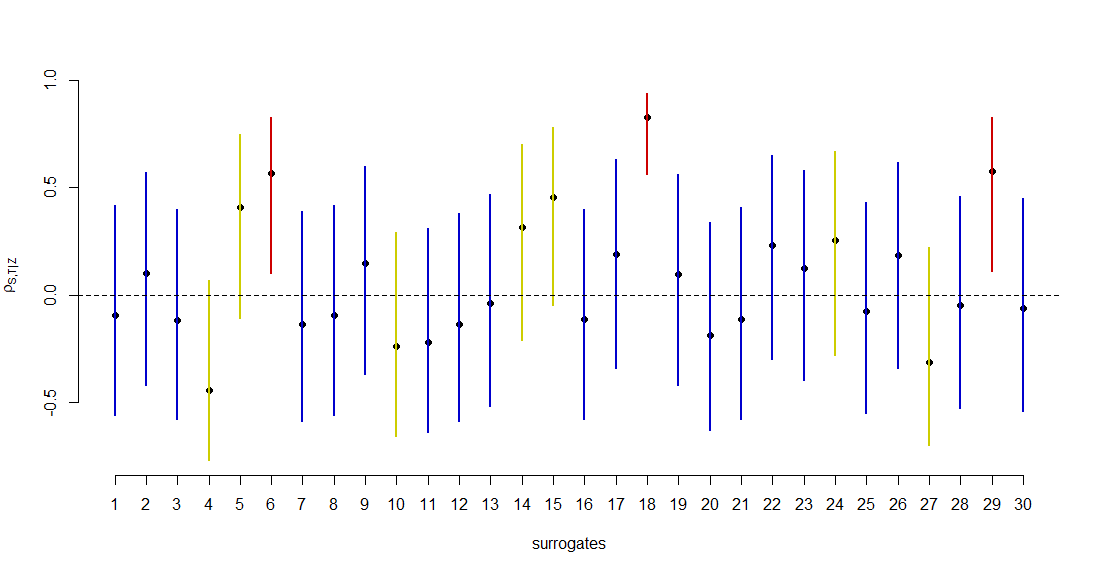
\includegraphics[scale=0.5]{adjustedassociationplot.png}
\caption{ \tiny Adjusted Association Plot. Top 3 surrogates in red, next 7 including 4 in yellow and others in blue.}
\end{figure}

\tiny
\begin{itemize}
\item Surrogates 6, 18 and 29 have the highest adjusted association, implying they are good surrogates by this approach.
\item surrogate 4 appears to contain information not present in other surrogaes since its adjusted association and confidence interval goes entirely in the opposite direction. 
\end{itemize}

\end{frame}

\begin{frame}{Causal Inference Results}
\tiny
\begin{table}[H]
\centering
\begin{tabular}{rrrrrrrrrr}
  \hline
S & $\rho_0$ & LCI0 & UCI0 & $\rho_1$ & LCI1 & UCI1 & ICA & lR & UR \\ 
  \hline
 \alert{18} & 0.84 & 0.60 & 0.94 & 0.81 & 0.52 & 0.93 & 0.91 & -0.76 & 1.00 \\ 
    \alert{6} & 0.57 & 0.11 & 0.83 & 0.56 & 0.10 & 0.83 & 0.84 & -0.96 & 1.00 \\ 
   \alert{15} & 0.20 & -0.33 & 0.63 & 0.79 & 0.49 & 0.93 & 0.83 & -0.91 & 0.93 \\ 
   \alert{17} & 0.21 & -0.32 & 0.64 & 0.14 & -0.39 & 0.59 & 0.74 & -1.00 & 1.00 \\ 
   \alert{19} & 0.00 & -0.49 & 0.50 & 0.21 & -0.32 & 0.64 & 0.70 & -0.99 & 0.99 \\ 
   \alert{24} & -0.10 & -0.57 & 0.41 & 0.81 & 0.52 & 0.93 & 0.69 & -0.85 & 0.86 \\ 
   \alert{29} & 0.85 & 0.60 & 0.95 & -0.11 & -0.57 & 0.41 & 0.67 & -0.81 & 0.84 \\ 
   \alert{14} & 0.32 & -0.21 & 0.70 & 0.32 & -0.21 & 0.70 & 0.63 & -0.99 & 1.00 \\ 
    \alert{5} & -0.16 & -0.60 & 0.37 & 0.88 & 0.67 & 0.96 & 0.60 & -0.73 & 0.80 \\ 
   \alert{22} & 0.43 & -0.09 & 0.76 & -0.10 & -0.57 & 0.42 & 0.58 & -0.96 & 0.95 \\ 
    2 & 0.32 & -0.21 & 0.70 & -0.01 & -0.50 & 0.49 & 0.57 & -0.98 & 0.98 \\ 
   20 & -0.51 & -0.80 & -0.02 & 0.73 & 0.37 & 0.90 & 0.53 & -0.75 & 0.77 \\ 
   23 & 0.06 & -0.45 & 0.54 & 0.30 & -0.23 & 0.69 & 0.52 & -0.99 & 0.98 \\ 
    8 & -0.52 & -0.81 & -0.03 & 0.37 & -0.15 & 0.73 & 0.52 & -0.87 & 0.87 \\ 
   26 & 0.39 & -0.14 & 0.74 & -0.19 & -0.63 & 0.34 & 0.51 & -0.95 & 0.95 \\ 
   11 & -0.57 & -0.83 & -0.10 & 0.70 & 0.32 & 0.89 & 0.48 & -0.75 & 0.74 \\ 
    9 & 0.19 & -0.34 & 0.63 & 0.01 & -0.49 & 0.50 & 0.48 & -0.99 & 0.99 \\ 
    3 & 0.20 & -0.33 & 0.63 & -0.38 & -0.74 & 0.14 & 0.34 & -0.94 & 0.94 \\ 
   30 & 0.28 & -0.25 & 0.68 & -0.28 & -0.68 & 0.25 & 0.33 & -0.95 & 0.95 \\ 
   28 & 0.02 & -0.48 & 0.51 & -0.23 & -0.65 & 0.30 & 0.31 & -0.99 & 0.99 \\ 
    1 & 0.01 & -0.49 & 0.50 & -0.24 & -0.66 & 0.29 & 0.30 & -0.99 & 0.98 \\ 
   12 & -0.27 & -0.67 & 0.26 & 0.09 & -0.43 & 0.56 & 0.28 & -0.97 & 0.98 \\ 
   13 & 0.29 & -0.24 & 0.69 & -0.50 & -0.80 & -0.00 & 0.17 & -0.91 & 0.90 \\ 
    7 & 0.06 & -0.45 & 0.54 & -0.32 & -0.70 & 0.21 & 0.14 & -0.98 & 0.97 \\ 
   16 & -0.10 & -0.57 & 0.42 & -0.15 & -0.60 & 0.37 & 0.13 & -0.99 & 0.99 \\ 
   25 & 0.18 & -0.34 & 0.62 & -0.47 & -0.78 & 0.04 & 0.05 & -0.93 & 0.93 \\ 
   27 & -0.44 & -0.77 & 0.07 & 0.16 & -0.37 & 0.61 & 0.05 & -0.95 & 0.95 \\ 
   10 & -0.48 & -0.79 & 0.02 & 0.18 & -0.35 & 0.62 & 0.05 & -0.93 & 0.94 \\ 
   21 & 0.12 & -0.40 & 0.58 & -0.47 & -0.78 & 0.03 & 0.03 & -0.95 & 0.94 \\ 
    \alert{4} & -0.49 & -0.79 & 0.01 & -0.59 & -0.84 & -0.13 & -0.79 & -1.00 & 0.97 \\ 
   \hline
\end{tabular}
\end{table}

\end{frame}

\begin{frame}{Causal Inference Results Cont:}
\begin{figure}[H]
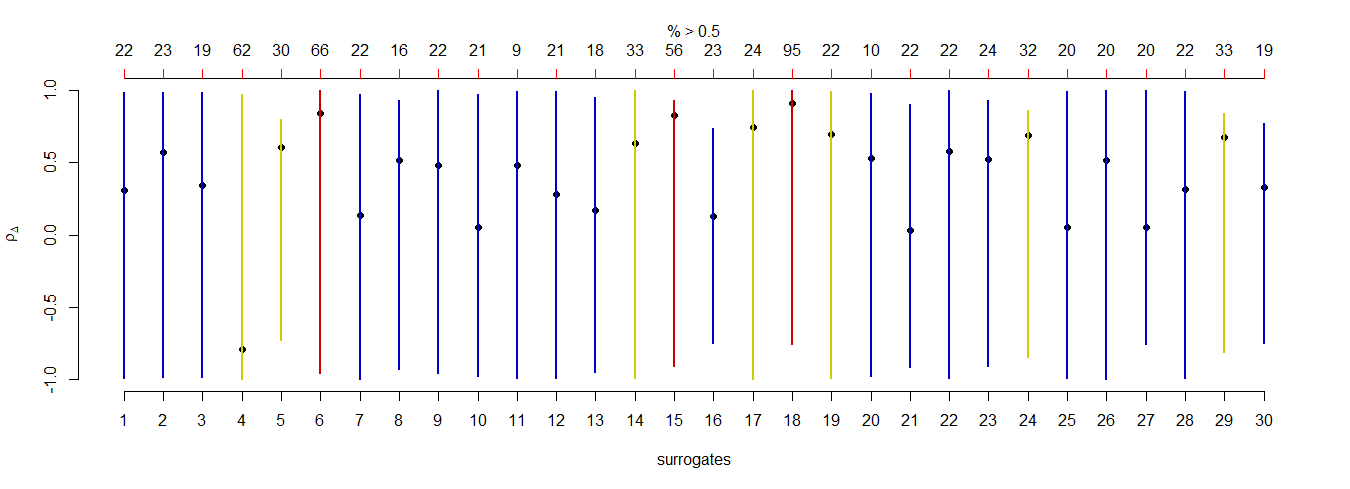
\includegraphics[scale=0.35]{icaplotRange.png}
\caption{\tiny ICA and Range plus percentage of ICA > 0.5}
\end{figure}
\tiny
\begin{itemize}
\item Surrogates 6, 15 and 18 have the highest ICA values but 18 has the least range amongst these 3 surrogates.
\item surrogate 4 appears to contain information not present in other surrogaes since its ICA values goes entirely in the opposite direction. 
\end{itemize}
\end{frame}

\section{Multivariate Surrogates}

\begin{frame}{Multivariate Joint Modelling}
\tiny
Since surrogates 18 was promising, only a combination of surrogate 18 and other surrogates will be considered.
\begin{table}[H]
\centering
\begin{tabular}{ccccccc}
  \hline
S & MAA & MAA\_CLI & MAA\_CLU & AMAA & AMAA\_CLI & AMAA\_CLU \\ 
  \hline
\alert{18,22} & 0.77 & 0.55 & 0.99 & 0.73 & 0.49 & 0.98 \\ 
  \alert{18,4} & 0.75 & 0.52 & 0.99 & 0.71 & 0.45 & 0.98 \\ 
  \alert{18,6} & 0.75 & 0.52 & 0.99 & 0.71 & 0.45 & 0.98 \\ 
  18,26 & 0.72 & 0.47 & 0.98 & 0.68 & 0.39 & 0.97 \\ 
  \alert{18,5} & 0.71 & 0.45 & 0.98 & 0.67 & 0.37 & 0.96 \\ 
  18,19 & 0.71 & 0.44 & 0.98 & 0.66 & 0.37 & 0.96 \\ 
  18,14 & 0.70 & 0.43 & 0.97 & 0.66 & 0.36 & 0.96 \\ 
  18,29 & 0.70 & 0.43 & 0.97 & 0.66 & 0.36 & 0.96 \\ 
  18,17 & 0.70 & 0.43 & 0.97 & 0.66 & 0.36 & 0.96 \\ 
  18,15 & 0.69 & 0.40 & 0.97 & 0.64 & 0.32 & 0.95 \\ 
  18,24 & 0.69 & 0.40 & 0.97 & 0.64 & 0.32 & 0.95 \\ 
   \hline
\end{tabular}
\caption{Adjusted and Multivariate Adjusted Association ranked by MAA values}
\end{table}
\tiny
\begin{itemize}
\item surrogates (18,6), (18,4) and (18,22) are the top 3 bivariate surrogates
\item surrogates 6, 4 and 22 added some more information to surrogate 18, since the $\rho^2_{adj}$ increased from 0.689 in the univariate case(i.e. 18 alone) to 0.77, 0.75 and 0.75 respectively.
\item the uncertainty about these three bivariate surogates appears to be within the same range(see plot on the next slide).

\end{itemize}

\end{frame}

\begin{frame}{Multivariate Adjusted Association(Cont:)}

\begin{figure}[H]
\includegraphics[scale=0.5]{mjointmodel.png}
\caption{\tiny Multivariate Adjusted Association, top 3 in red.}
\end{figure}
\end{frame}

\begin{frame}{Multivariate Causal Inference}
\tiny
\begin{table}[H]
\centering
\begin{tabular}{cccccccc}
  \hline
S & MMICA & lower\_MMICA & upper\_MMICA & MAMICA & lower\_MAMICA & upper\_MAMICA \\ 
  \hline
\alert{S18,S22} & 0.83 & 0.17 & 0.96 & 0.80 & 0.04 & 0.95 \\ 
\alert{S18,S6} & 0.81 & 0.22 & 0.98 & 0.78 & 0.09 & 0.98 \\ 
\alert{S18,S5} & 0.80 & 0.32 & 0.97 & 0.77 & 0.22 & 0.97 \\ 
\alert{S18,S4} & 0.79 & 0.42 & 0.97 & 0.76 & 0.33 & 0.97 \\ 
S18,S29 & 0.78 & 0.30 & 0.97 & 0.74 & 0.19 & 0.97 \\ 
S18,S19 & 0.76 & 0.23 & 0.99 & 0.73 & 0.12 & 0.98 \\ 
S18,S14 & 0.76 & 0.14 & 0.97 & 0.73 & 0.00 & 0.97 \\ 
S18,S17 & 0.76 & 0.13 & 0.96 & 0.72 & -0.01 & 0.95 \\ 
S18,S26 & 0.75 & 0.29 & 0.98 & 0.71 & 0.19 & 0.97 \\ 
S18,S15 & 0.75 & 0.21 & 0.97 & 0.71 & 0.09 & 0.97 \\ 
S18,S24 & 0.72 & 0.24 & 0.97 & 0.67 & 0.13 & 0.96 \\ 
   \hline
\end{tabular}
\caption{MMICA and Range}
\end{table}

\tiny
\begin{itemize}
\item addition of other surrogate 22 improved ICA value for surrogate 18 but the range of the bivariate surrogates 18 and 22 is more than the other top bivariate surrogates
\item again surrogate 4 improves surrogates 18 by narrowing down the range of ICA values compared to addition of other surrogates to surrogate 18. 
\end{itemize}

\end{frame}

\begin{frame}{MICA Plots}
\begin{figure}[H]
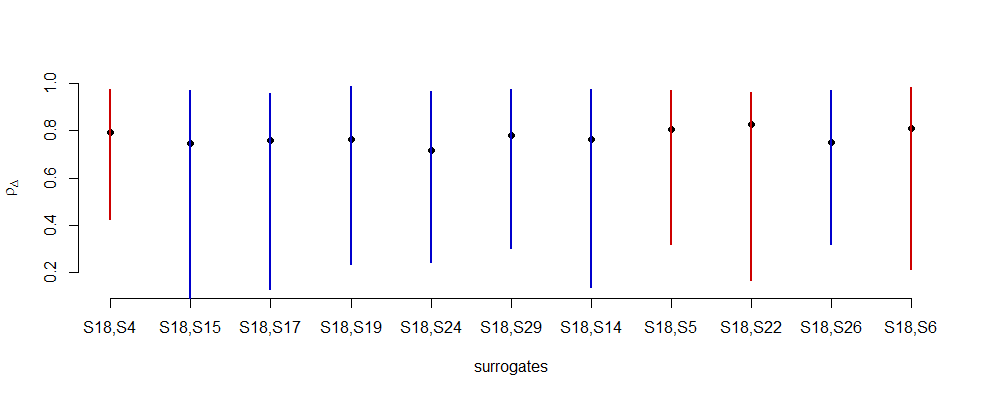
\includegraphics[scale=0.35]{MICAplot.png}
\caption{\tiny ICA and Range plus}
\end{figure}
\end{frame}


\end{document}
